\section{Interfejs graficzny}
W celu stworzenia GUI wykorzystano biblioteki \textit{Qt}. Interfejs graficzny został zaprojektowany z wykorzystaniem programu \textit{QtDesigner}.

\subsection{Wykorzystane klasy}
Tworząc interfejs wykorzystano biblioteki:

\begin{itemize}
\item \textbf{QGraphicsScene} - biblioteka pozwalająca na stworzenie obiektu reprezentującego dwuwymiarową scenę graficzną, na scenie można tworzyć i umieszczać obiekty (pojedyncze piksele, wieloboki), obiekty można poddawać transformacji przy pomocy klasy \textit{QTransform},
\item \textbf{QGraphicsView} - biblioteka, przy pomocy której można wizualizować zawartość sceny utworzonej z wykorzystaniem klasy \textit{QGraphicsScene}.
 \end{itemize}

\subsection{Interfejs programu}
Do dyspozycji użytkownika udostępniono interfejs użytkownika pozwalający sterować symulacją. 

\begin{figure}[!htp]
  \centering
  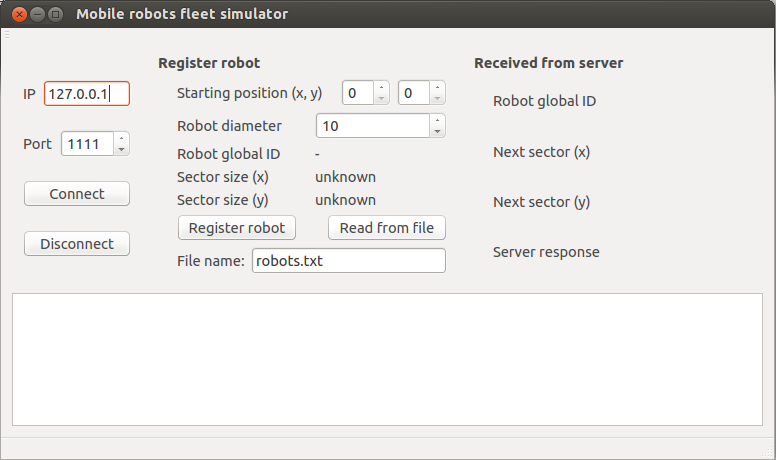
\includegraphics[width=0.8\textwidth]{img/klient.png}
  \caption{Widok interfejsu programu.}
  \label{fig:interfejs}
\end{figure}


	\subsubsection{Połączenie w serwerem}

		Połączenie z serwerem ustala się w panelu bocznym. Należy zadeklarować adres IP serwera i port po którym będzie się obywało połączenie. Widok interfejsu przedstawiono na rysunku \ref{fig:polaczenie}.
		
		\begin{figure}[!htp]
  			\centering
		  	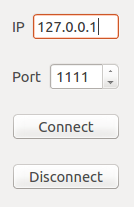
\includegraphics[width=0.2\textwidth]{img/polaczenie.png}
  			\caption{Widok interfejsu do połączenia z serwerem.}
  			\label{fig:polaczenie}
		\end{figure}
		
		Próba połączenia następuje po naciśnięciu przycisku \textit{Connect}. Zerwanie połączenia z serwerem odbywa się po naciśnięciu przycisku \textit{Disconnect}.
	
	\subsubsection{Rejestracja robotów}
	
	Rejestrowanie robotów może odbywać się na dwa sposoby:
	\begin{itemize}
		\item odczyt z pliku wszystkich robotów,
		\item ręczna rejestracja robota.
	\end{itemize}
	
		\begin{figure}[!htp]
  			\centering
		  	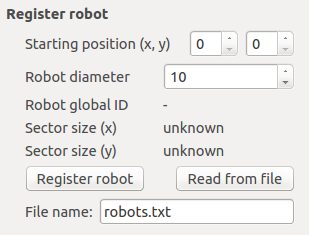
\includegraphics[width=0.4\textwidth]{img/rejestracja.png}
  			\caption{Widok interfejsu do rejestracji robotów.}
  			\label{fig:rejestracja}
		\end{figure}
	
	
	W pliku zawierającym rejestrowane roboty należy podać komórkę startową robota i rozmiar robota.
	Do ręcznej rejestracji został udostępniony panel umożliwiający zadanie pozycji początkowej i rozmiaru robota. Widok interfejsu przedstawiono na rysunku \ref{fig:rejestracja}.
	
	Po dokonanej rejestracji otrzymujemy informację zwrotną o przydzieleniu globalnego id robota.
	
	\subsubsection{Informowanie o otrzymanych sygnałach}
	
	W prawym panelu użytkownika wyświetlają się informacje o obecnie otrzymywanych zezwoleniach od serwera.	 Widok interfejsu przedstawiono na rysunku \ref{fig:zdarzenia}.
	
		\begin{figure}[!htp]
  			\centering
		  	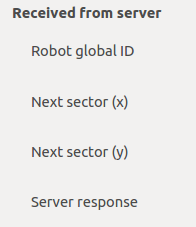
\includegraphics[width=0.2\textwidth]{img/sygnaly.png}
  			\caption{Widok interfejsu do informowania o przychodzących zdarzeniach.}
  			\label{fig:zdarzenia}
		\end{figure}
	
	\subsubsection{Wizualizacja pracy robotów}
	
	W dole okna programu jest wyświetlana scena pracy robotów. Widok interfejsu przedstawiono na rysunku \ref{fig:wizualizacja}.
	
		\begin{figure}[!htp]
  			\centering
		  	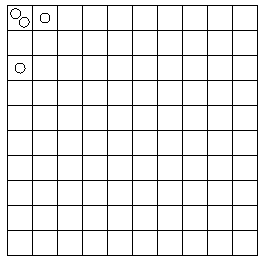
\includegraphics[width=0.3\textwidth]{img/wizualizacja.png}
  			\caption{Widok interfejsu do wizualizacji robotów.}
  			\label{fig:wizualizacja}
		\end{figure}



\begin{figure}[!htp]
  \centering
  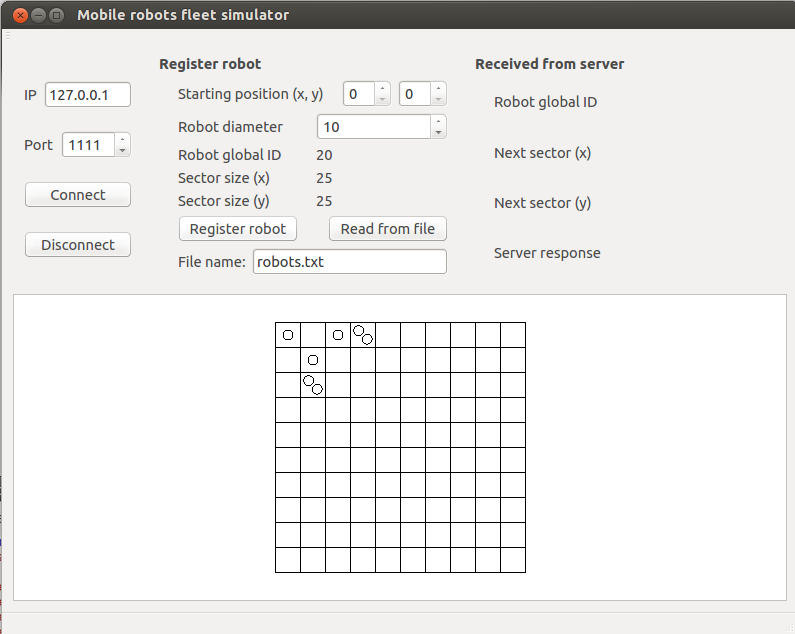
\includegraphics[width=0.8\textwidth]{img/klient_robot.png}
  \caption{Widok interfejsu programu po zarejestrowaniu robotów.}
  \label{fig:int_rej}
\end{figure}